\section{Preliminary Study}
\label{sec:A}
We show the accuracy-rank trade-offs on MRPC, RTE, and CoLA in \figref{fig:pre}~(CoLA is additionally included compared to the main body of the paper). The observation on CoLA is similar to MRPC/RTE: first-order unstructured pruning can extract subnetworks that are most accurate while having the lowest average matrix rank, which lays the crucial foundation of later factorization.

%\begin{theorem}
%	Let $t_i$ and $t_{j}$ where $t_{i}\geq t_{j}$ denote the time steps at which two different checkpoints are saved; Let $R(f_{\bm{\theta}^{(t\leftarrow t_i)}})$ and $R(f_{\bm{\theta}^{(t\leftarrow t_j)}})$ denote the expected generalization error of models learned from two checkpoints $\bm{\theta}^{(t_i)}$ and $\bm{\theta}^{(t_j)}$; Let n denotes the size of training data; $|\cdot|_{\text{C}}$ denotes a function class capacity measure like VC-dimension. Based on previous expositions on VC theory, the following asymptotic generalization bound holds:
%	\begin{align}\nonumber
	%		R(f_{\bm{\theta}^{(t\leftarrow t_i)}})&=R(f_{\bm{\theta}^{(t\leftarrow t_i)}})-R(f_{\bm{\theta}^{(t_i)}})+R(f_{\bm{\theta}^{(t_i)}}) \\ \nonumber
	%				&\leq O(\frac{|f_{\bm{\theta}^{(t)}}|_{\text{C}}}{n^{\alpha_{i}}})+ \epsilon_{t,t_i} + R(f_{\bm{\theta}^{(t_i)}}) \\ \nonumber 
	%				&=  \underbrace{O(\frac{|f_{\bm{\theta}^{(t)}}|_{\text{C}}}{n^{\alpha_{i}}}) + \underset{\bm{\theta}^{(t)}\in \mathcal{F}_{\bm{\theta}^{(t\leftarrow t_i)}}}{\inf}R(f_{\bm{\theta}^{(t)}})}_{bound(f_{\bm{\theta}^{(t\leftarrow t_i)}})} \\ \nonumber
	%		R(f_{\bm{\theta}^{(t\leftarrow t_j)}})&=R(f_{\bm{\theta}^{(t\leftarrow t_j)}})-R(f_{\bm{\theta}^{(t_j)}})+R(f_{\bm{\theta}^{(t_j)}}) \\ \nonumber
	%&\leq O(\frac{|f_{\bm{\theta}^{(t)}}|_{\text{C}}}{n^{\alpha_{j}}})+ \epsilon_{t,t_j} + R(f_{\bm{\theta}^{(t_j)}}) \\ \nonumber 
	%&=  \underbrace{O(\frac{|f_{\bm{\theta}^{(t)}}|_{\text{C}}}{n^{\alpha_{j}}}) + \underset{\bm{\theta}^{(t)}\in \mathcal{F}_{\bm{\theta}^{(t\leftarrow t_j)}}}{\inf}R(f_{\bm{\theta}^{(t)}})}_{bound(f_{\bm{\theta}^{(t\leftarrow t_j)}})}
	%	\end{align}
%where $\epsilon_{t,ti}$ is the approximation error of function class $\mathcal{F}_{\bm{\theta}^{(t\leftarrow t_i)}}$ with respect to $f_{\bm{\theta}^{(t_i)}}$. $\epsilon_{t,tj}$ is defined in analogy.
%	Because: (1) $\bm{\theta}^{(t_i)}$ is a later checkpoint with higher sparsity than $\bm{\theta}^{(t_j)}$, we have the learning speed $1\geq \alpha_{i}\geq \alpha_{j}\geq \frac{1}{2}$; (2) $\bm{\theta}^{(t_i)}$ has lower generalization error than $\bm{\theta}^{(t_j)}$, we have the following inequality holds with large probability:
%	\begin{align}\nonumber
	%		bound(f_{\bm{\theta}^{(t\leftarrow t_i)}}) \leq bound(f_{\bm{\theta}^{(t\leftarrow t_j)}})
	%	\end{align}
%\end{theorem}

\begin{figure*}[t]
	\centering
	\scalebox{0.285}{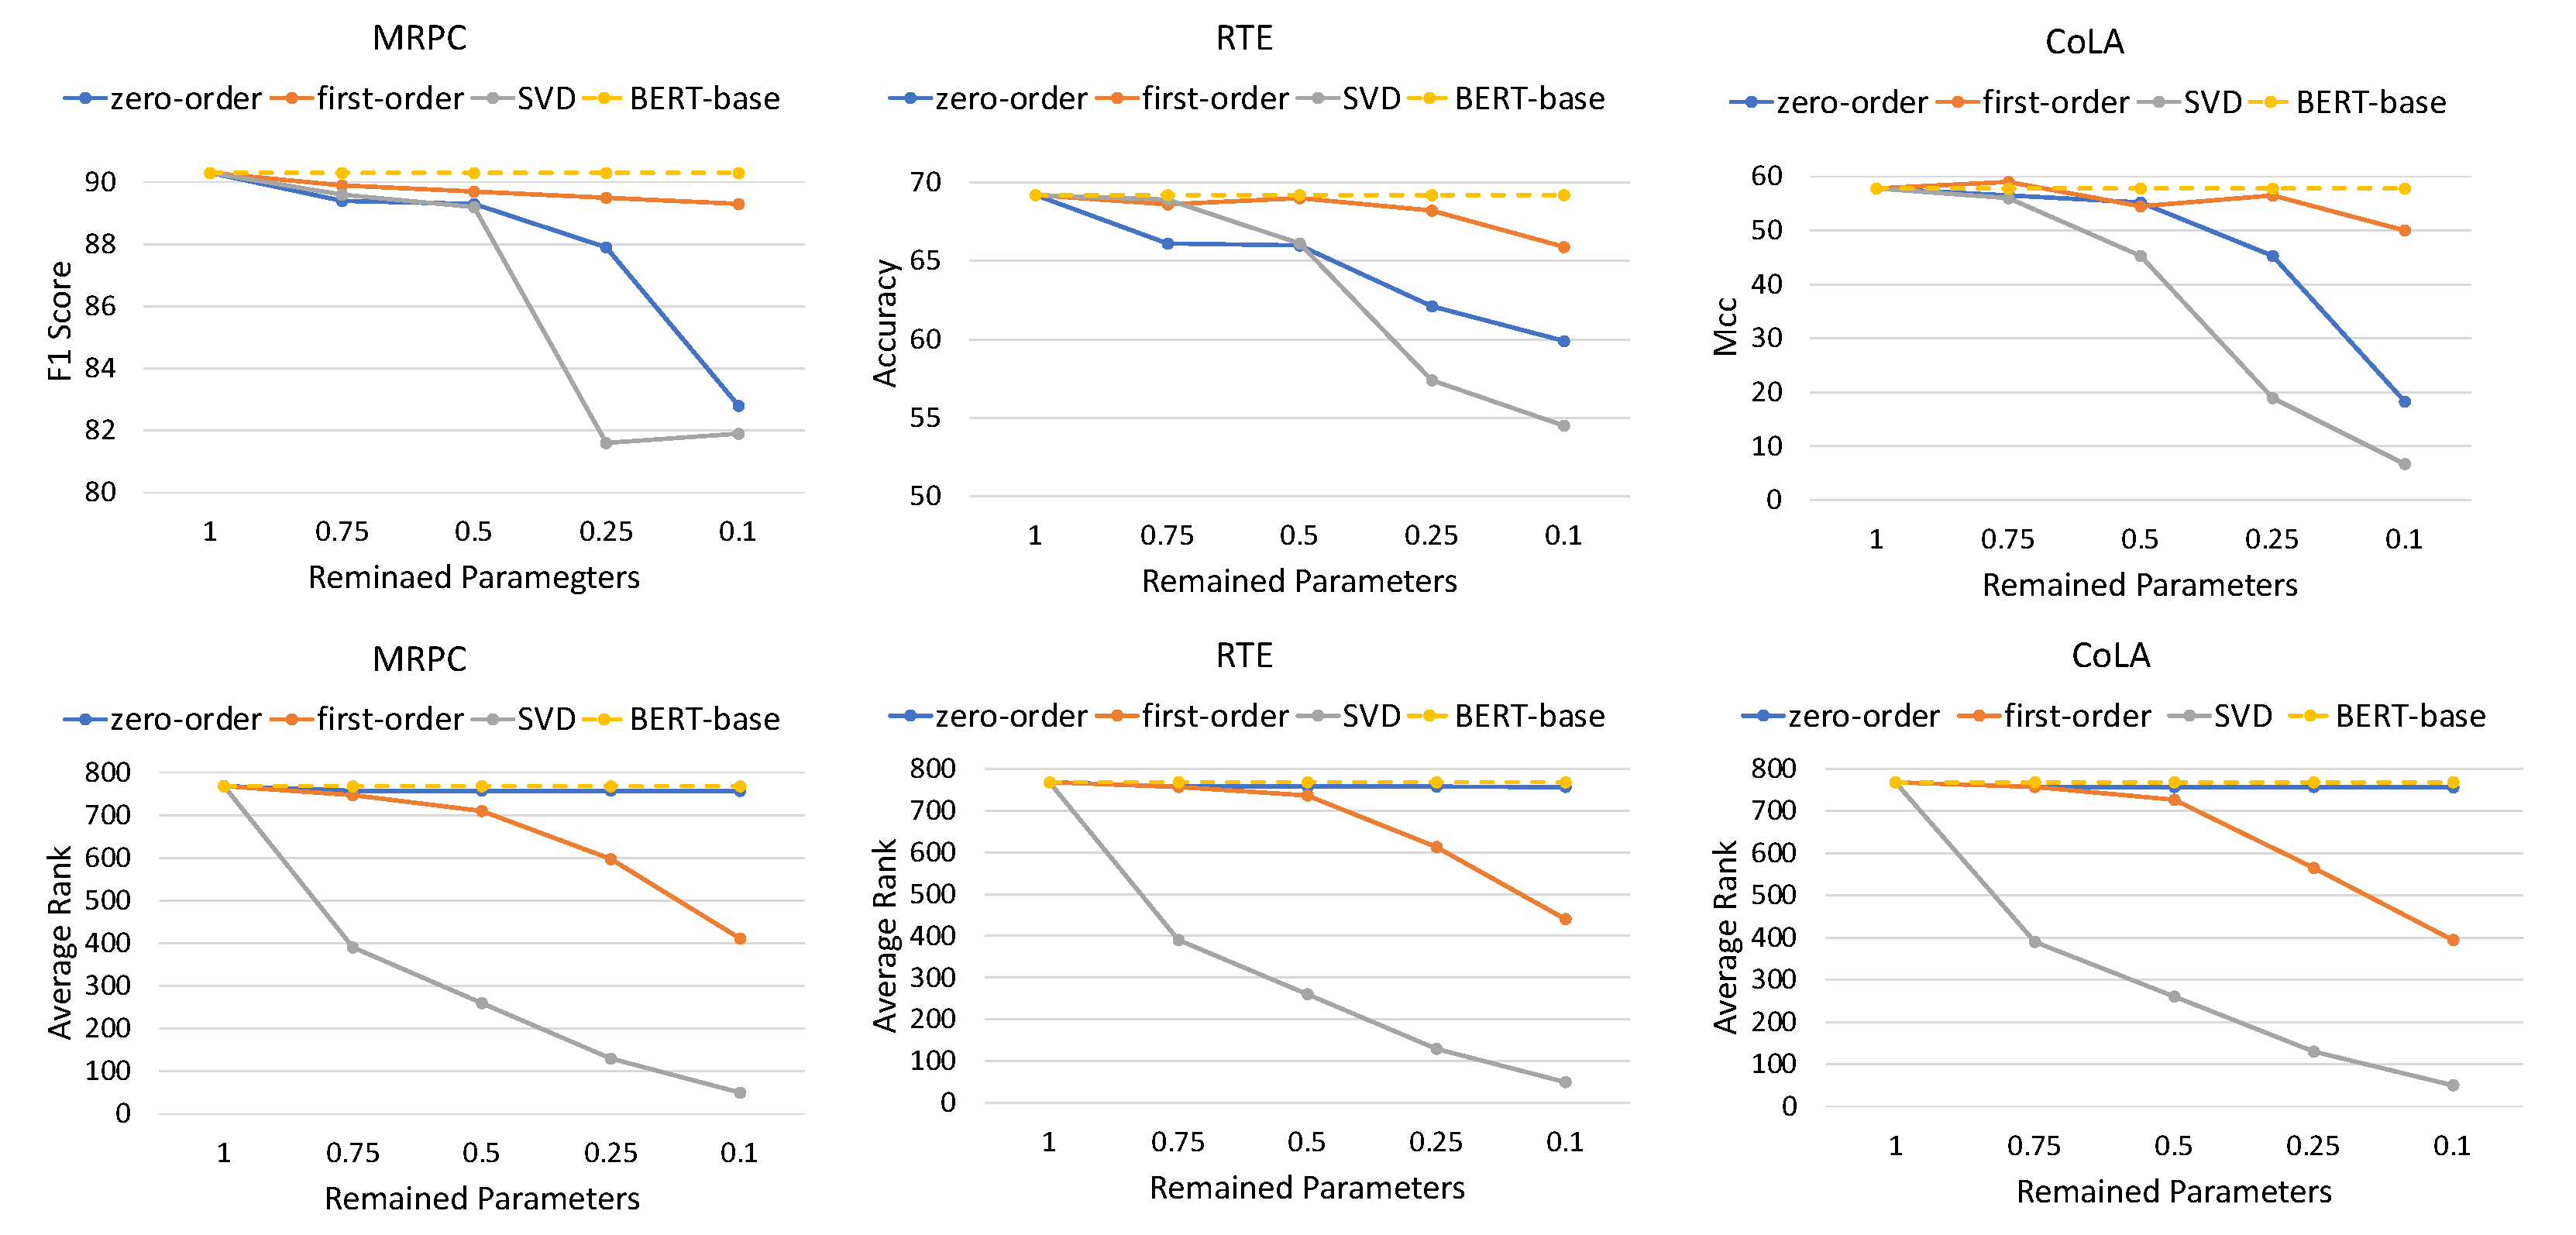
\includegraphics{./figures/pre_new.pdf}}
	\caption{Task accuracy (top half) and average matrix rank (bottom half) v.s. percentage of original parameters retained. The dashed line indicates the performance/rank upper bound by fine-tuning the full-scale BERT-base model.}
	\label{fig:pre}
\end{figure*}